%----------------------------------------------------------------------------------------
%   PACKAGES AND OTHER DOCUMENT CONFIGURATIONS
%----------------------------------------------------------------------------------------

\documentclass[
10pt, % Main document font size
a4paper, % Paper type, use 'letterpaper' for US Letter paper
oneside, % One page layout (no page indentation)
%twoside, % Two page layout (page indentation for binding and different headers)
headinclude,footinclude, % Extra spacing for the header and footer
BCOR5mm, % Binding correction
]{scrartcl}

\usepackage[utf8]{inputenc}
\usepackage[english]{babel}

\usepackage{geometry}
\geometry{textheight = 22cm}

\usepackage{comment}

\usepackage{graphics,graphicx}
\graphicspath{ {./figures/} }
\usepackage{amsmath}
\usepackage{physics}

%%%%%%%%%%%%%%%%%%%%%%%%%%%%%%%%%%%%%%%%%
% Arsclassica Article
% Structure Specification File
%
% This file has been downloaded from:
% http://www.LaTeXTemplates.com
%
% Original author:
% Lorenzo Pantieri (http://www.lorenzopantieri.net) with extensive modifications by:
% Vel (vel@latextemplates.com)
%
% License:
% CC BY-NC-SA 3.0 (http://creativecommons.org/licenses/by-nc-sa/3.0/)
%
%%%%%%%%%%%%%%%%%%%%%%%%%%%%%%%%%%%%%%%%%

%----------------------------------------------------------------------------------------
%   REQUIRED PACKAGES
%----------------------------------------------------------------------------------------

\usepackage[
nochapters, % Turn off chapters since this is an article        
beramono, % Use the Bera Mono font for monospaced text (\texttt)
eulermath,% Use the Euler font for mathematics
pdfspacing, % Makes use of pdftex’ letter spacing capabilities via the microtype package
dottedtoc % Dotted lines leading to the page numbers in the table of contents
]{classicthesis} % The layout is based on the Classic Thesis style

\usepackage{arsclassica} % Modifies the Classic Thesis package

\usepackage[T1]{fontenc} % Use 8-bit encoding that has 256 glyphs

\usepackage[utf8]{inputenc} % Required for including letters with accents

\usepackage{graphicx} % Required for including images
\graphicspath{{Figures/}} % Set the default folder for images

\usepackage{enumitem} % Required for manipulating the whitespace between and within lists

\usepackage{lipsum} % Used for inserting dummy 'Lorem ipsum' text into the template

\usepackage{subfig} % Required for creating figures with multiple parts (subfigures)

\usepackage{amsmath,amssymb,amsthm} % For including math equations, theorems, symbols, etc

\usepackage{varioref} % More descriptive referencing

%----------------------------------------------------------------------------------------
%   THEOREM STYLES
%---------------------------------------------------------------------------------------

\theoremstyle{definition} % Define theorem styles here based on the definition style (used for definitions and examples)
\newtheorem{definition}{Definition}

\theoremstyle{plain} % Define theorem styles here based on the plain style (used for theorems, lemmas, propositions)
\newtheorem{theorem}{Theorem}

\theoremstyle{remark} % Define theorem styles here based on the remark style (used for remarks and notes)

%----------------------------------------------------------------------------------------
%   HYPERLINKS
%---------------------------------------------------------------------------------------

\hypersetup{
%draft, % Uncomment to remove all links (useful for printing in black and white)
colorlinks=true, breaklinks=true, bookmarks=true,bookmarksnumbered,
urlcolor=webbrown, linkcolor=RoyalBlue, citecolor=webgreen, % Link colors
pdftitle={}, % PDF title
pdfauthor={\textcopyright}, % PDF Author
pdfsubject={}, % PDF Subject
pdfkeywords={}, % PDF Keywords
pdfcreator={pdfLaTeX}, % PDF Creator
pdfproducer={LaTeX with hyperref and ClassicThesis} % PDF producer
} % Include the structure.tex file which specified the document structure and layout

%----------------------------------------------------------------------------------------
%   TITLE AND AUTHOR(S)
%----------------------------------------------------------------------------------------

\title{\normalfont\spacedallcaps{NOtes on Magnetic field design on PROCURE}} % The article title

%\subtitle{Subtitle} % Uncomment to display a subtitle

\author{\spacedlowsmallcaps{Bruno Ximenez} }% The article author(s) - author affiliations need to be specified in the AUTHOR AFFILIATIONS block

\date{31/01/2021} % An optional date to appear under the author(s)

\begin{document}
%----------------------------------------------------------------------------------------

%----------------------------------------------------------------------------------------
%   HEADERS
%----------------------------------------------------------------------------------------

\renewcommand{\sectionmark}[1]{\markright{\spacedlowsmallcaps{#1}}} % The header for all pages (oneside) or for even pages (twoside)
%\renewcommand{\subsectionmark}[1]{\markright{\thesubsection~#1}} % Uncomment when using the twoside option - this modifies the header on odd pages
\lehead{\mbox{\llap{\small\thepage\kern1em\color{halfgray} \vline}\color{halfgray}\hspace{0.5em}\rightmark\hfil}} % The header style

\pagestyle{scrheadings} % Enable the headers specified in this block


%----------------------------------------------------------------------------------------
%   TABLE OF CONTENTS & LISTS OF FIGURES AND TABLES
%----------------------------------------------------------------------------------------

\maketitle % Print the title/author/date block

\setcounter{tocdepth}{2} % Set the depth of the table of contents to show sections and subsections only

\tableofcontents % Print the table of contents

\listoffigures % Print the list of figures

\listoftables % Print the list of tables

\newpage

\section{$\vec{B}$ field configuration study}

Here is an initial investigation on the magnetic field produced by the under-vacuum coils designed for the PROCURE machine.
The setup is a pair of solenoids with about 5 turns. I consider here as an example, solenoids with radius of 40 mm and a distance between the two solenoids (in a Helmholtz configuration) of about 80 mm or the diameter of the coils. The current chosen to plot the graphs is 20 A. On figure \ref{helmholtz}. This setup generates a highly homogeneous magnetic field at the trapping site, which has a cubic volume with a length of  l = 30 $\times$ 5 $\mu$m $\approx$ 0.15 mm.



\begin{figure}[t]
    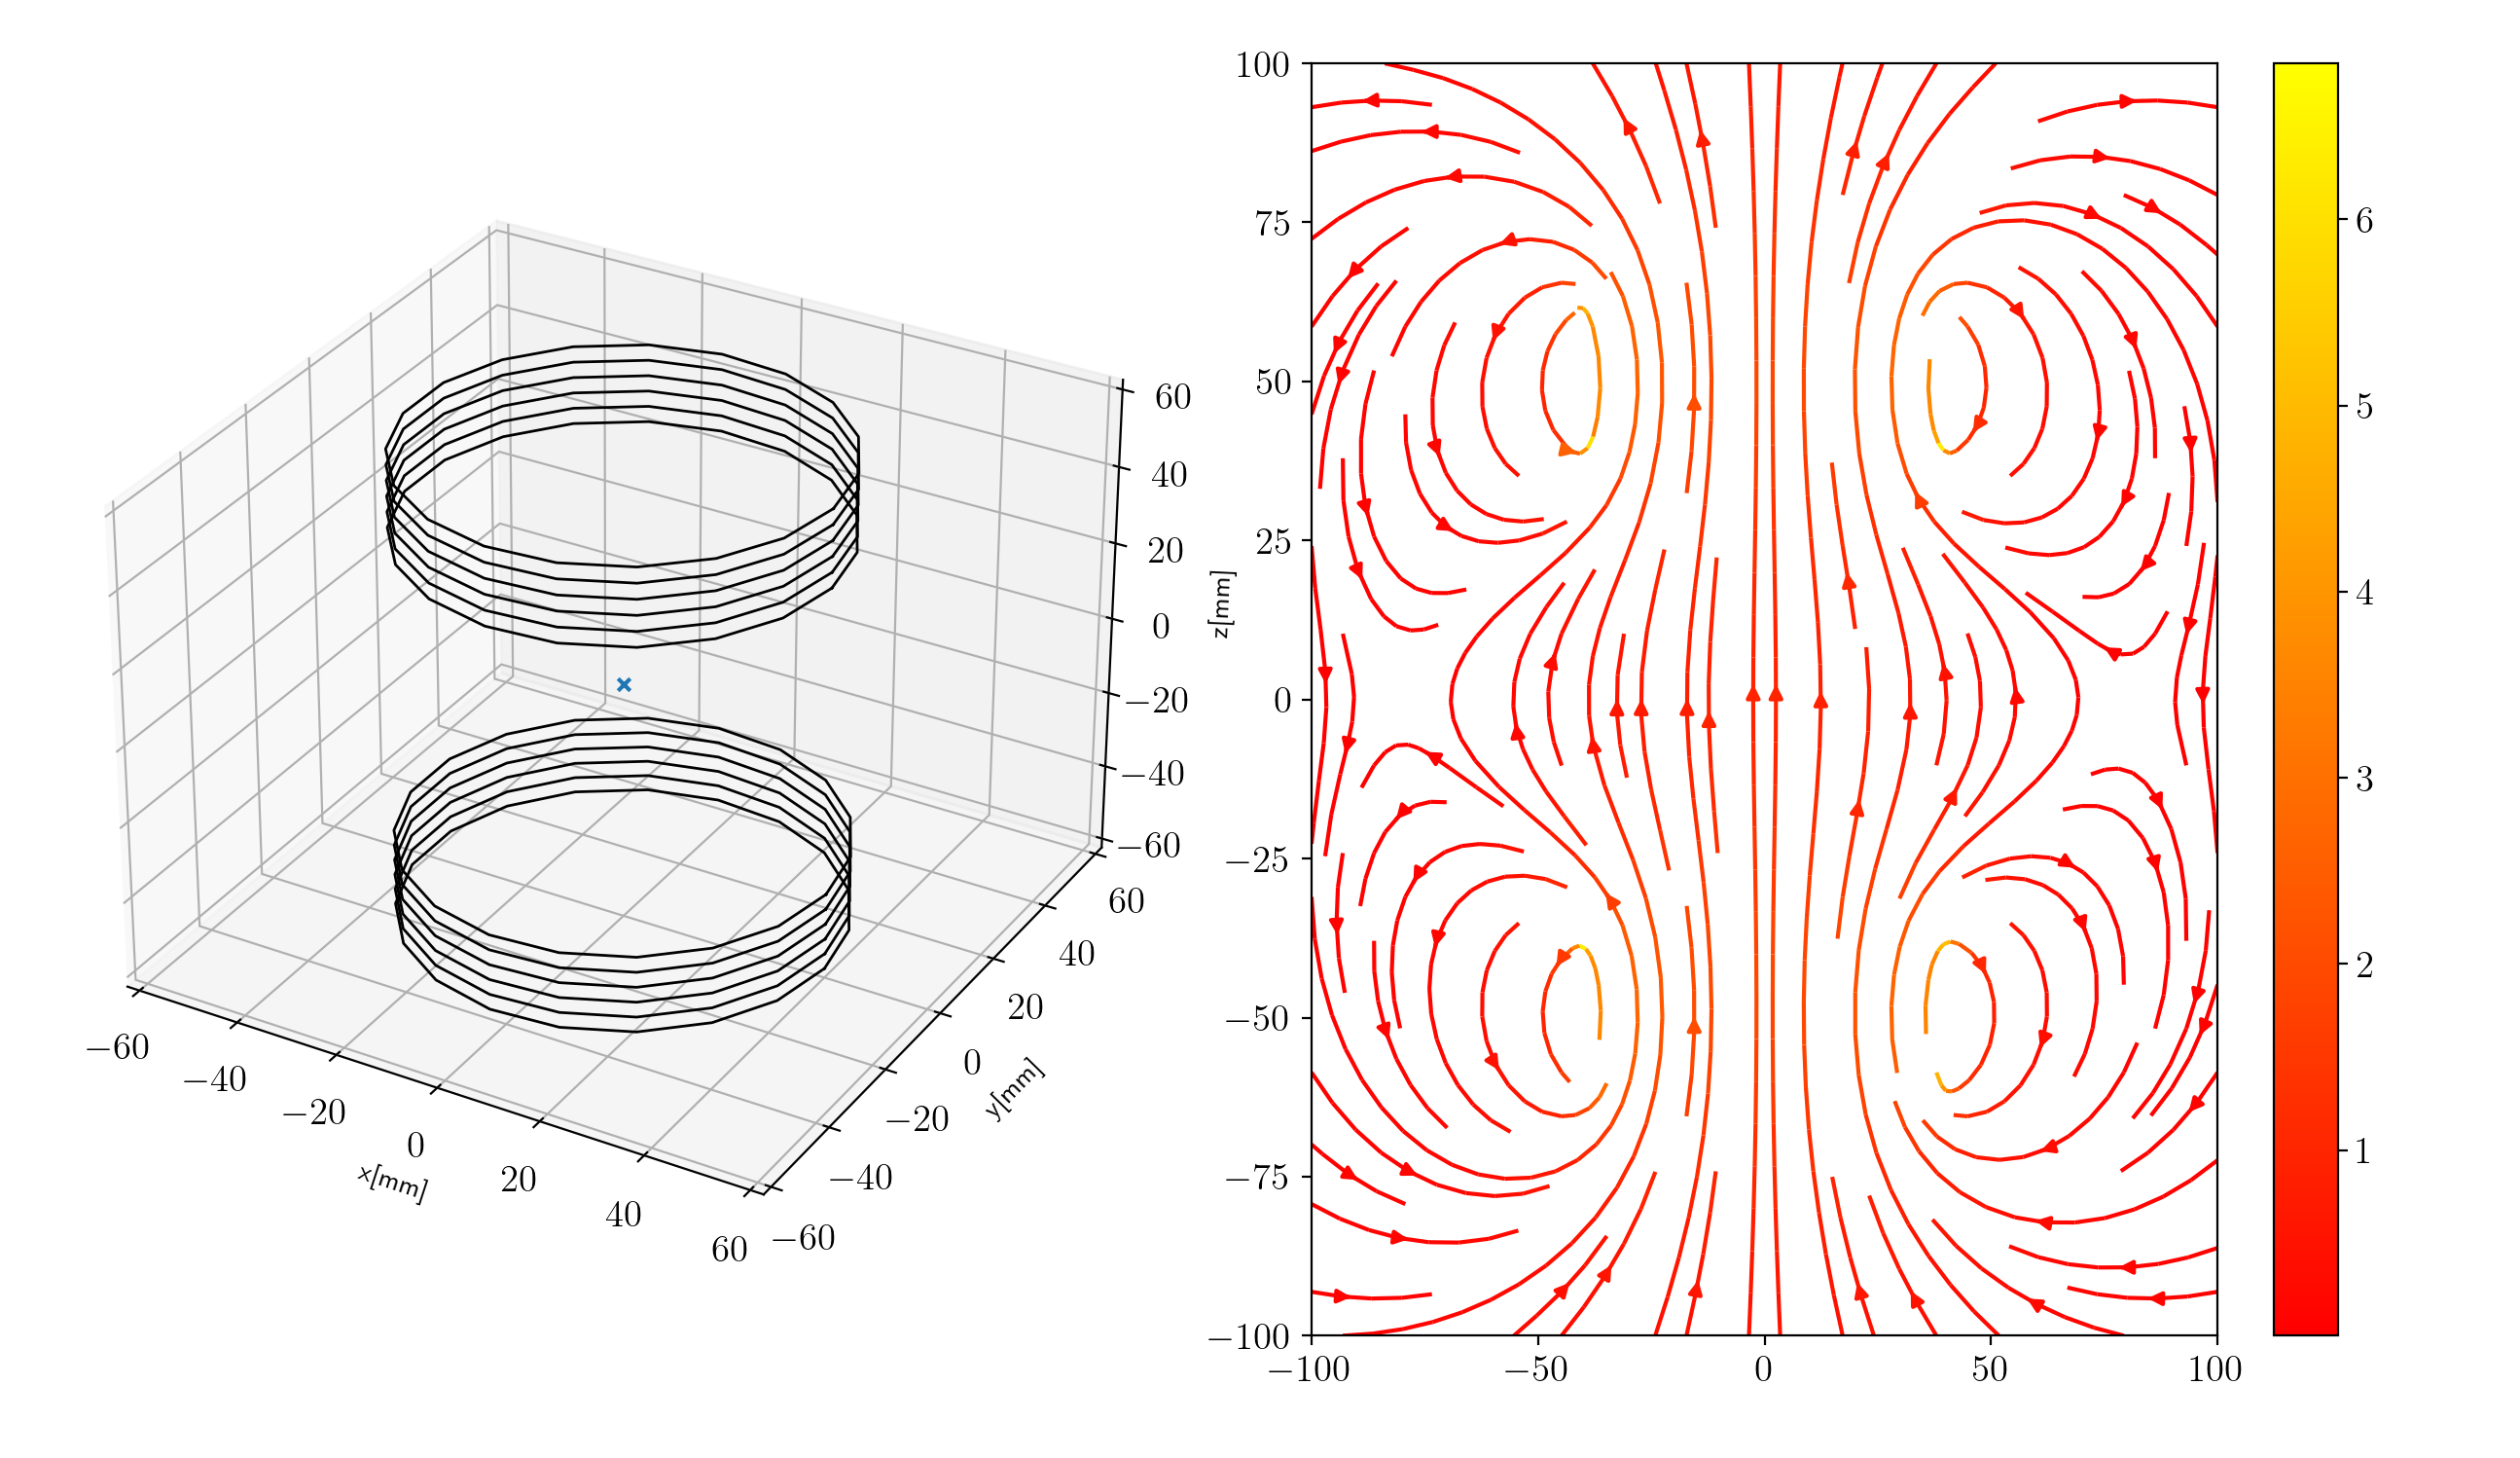
\includegraphics[width=\linewidth]{XZplane_6turns_20amps_radius40mm_d80}
    \centering
    \caption{The Helmholtz coils setup is representes on the left and on the right the line fields of the magnetic field on the XZ plane.}
    \label{helmholtz}
\end{figure}


For those parameters the magnetic field produced at the trap is on the order of 1 mT. Varying the distance between the coils by 2 mm leads to a change on the magnitude of the field on the order of $10^{-2}$ mT but the homegeneity is kept nearly the same, which is on the order of $\mu$T. Results are shown on figure \ref{dist}.


\begin{figure}[t]
    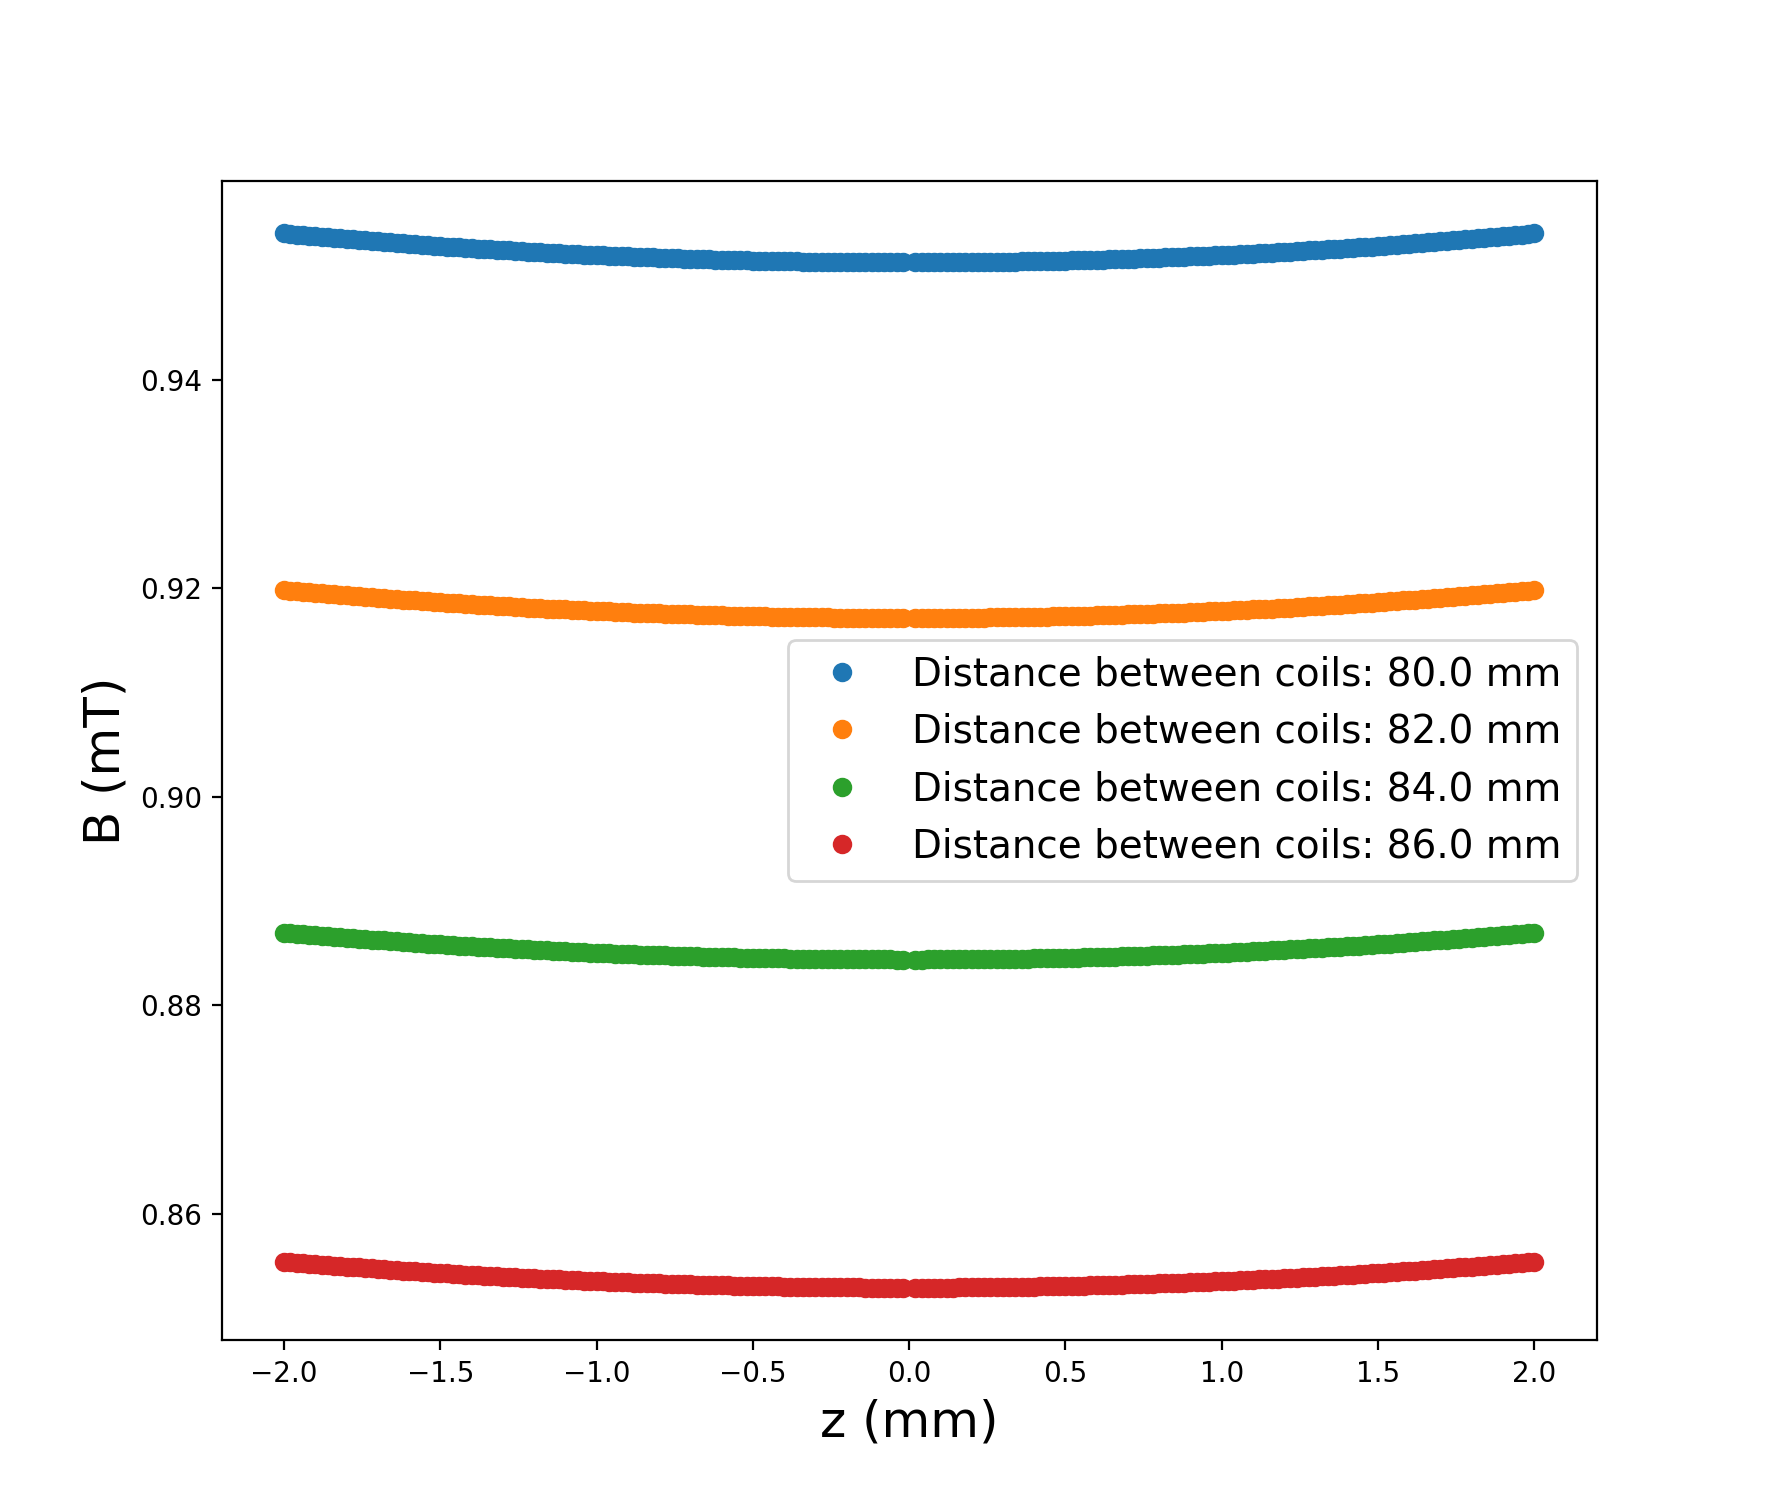
\includegraphics[width=\linewidth]{varying_distance_between_coils.png}
    \centering
    \caption{Magnitude of the magnetic field produced on the z-axis when varying the distance between the coils.}
    \label{dist}
\end{figure}

Next I tilt the one of the coils by about 10 degrees. On figure \ref{tilted_coil} is shown the geometric deformation and on figure \ref{tilted_coil_B} is the magnitude of the magnetic field on the z-axis. There is a shift on the minimum of the magnetic field and variations on the magnetic field on the level of $10^{-3}$ mT.

\begin{figure}[t]
    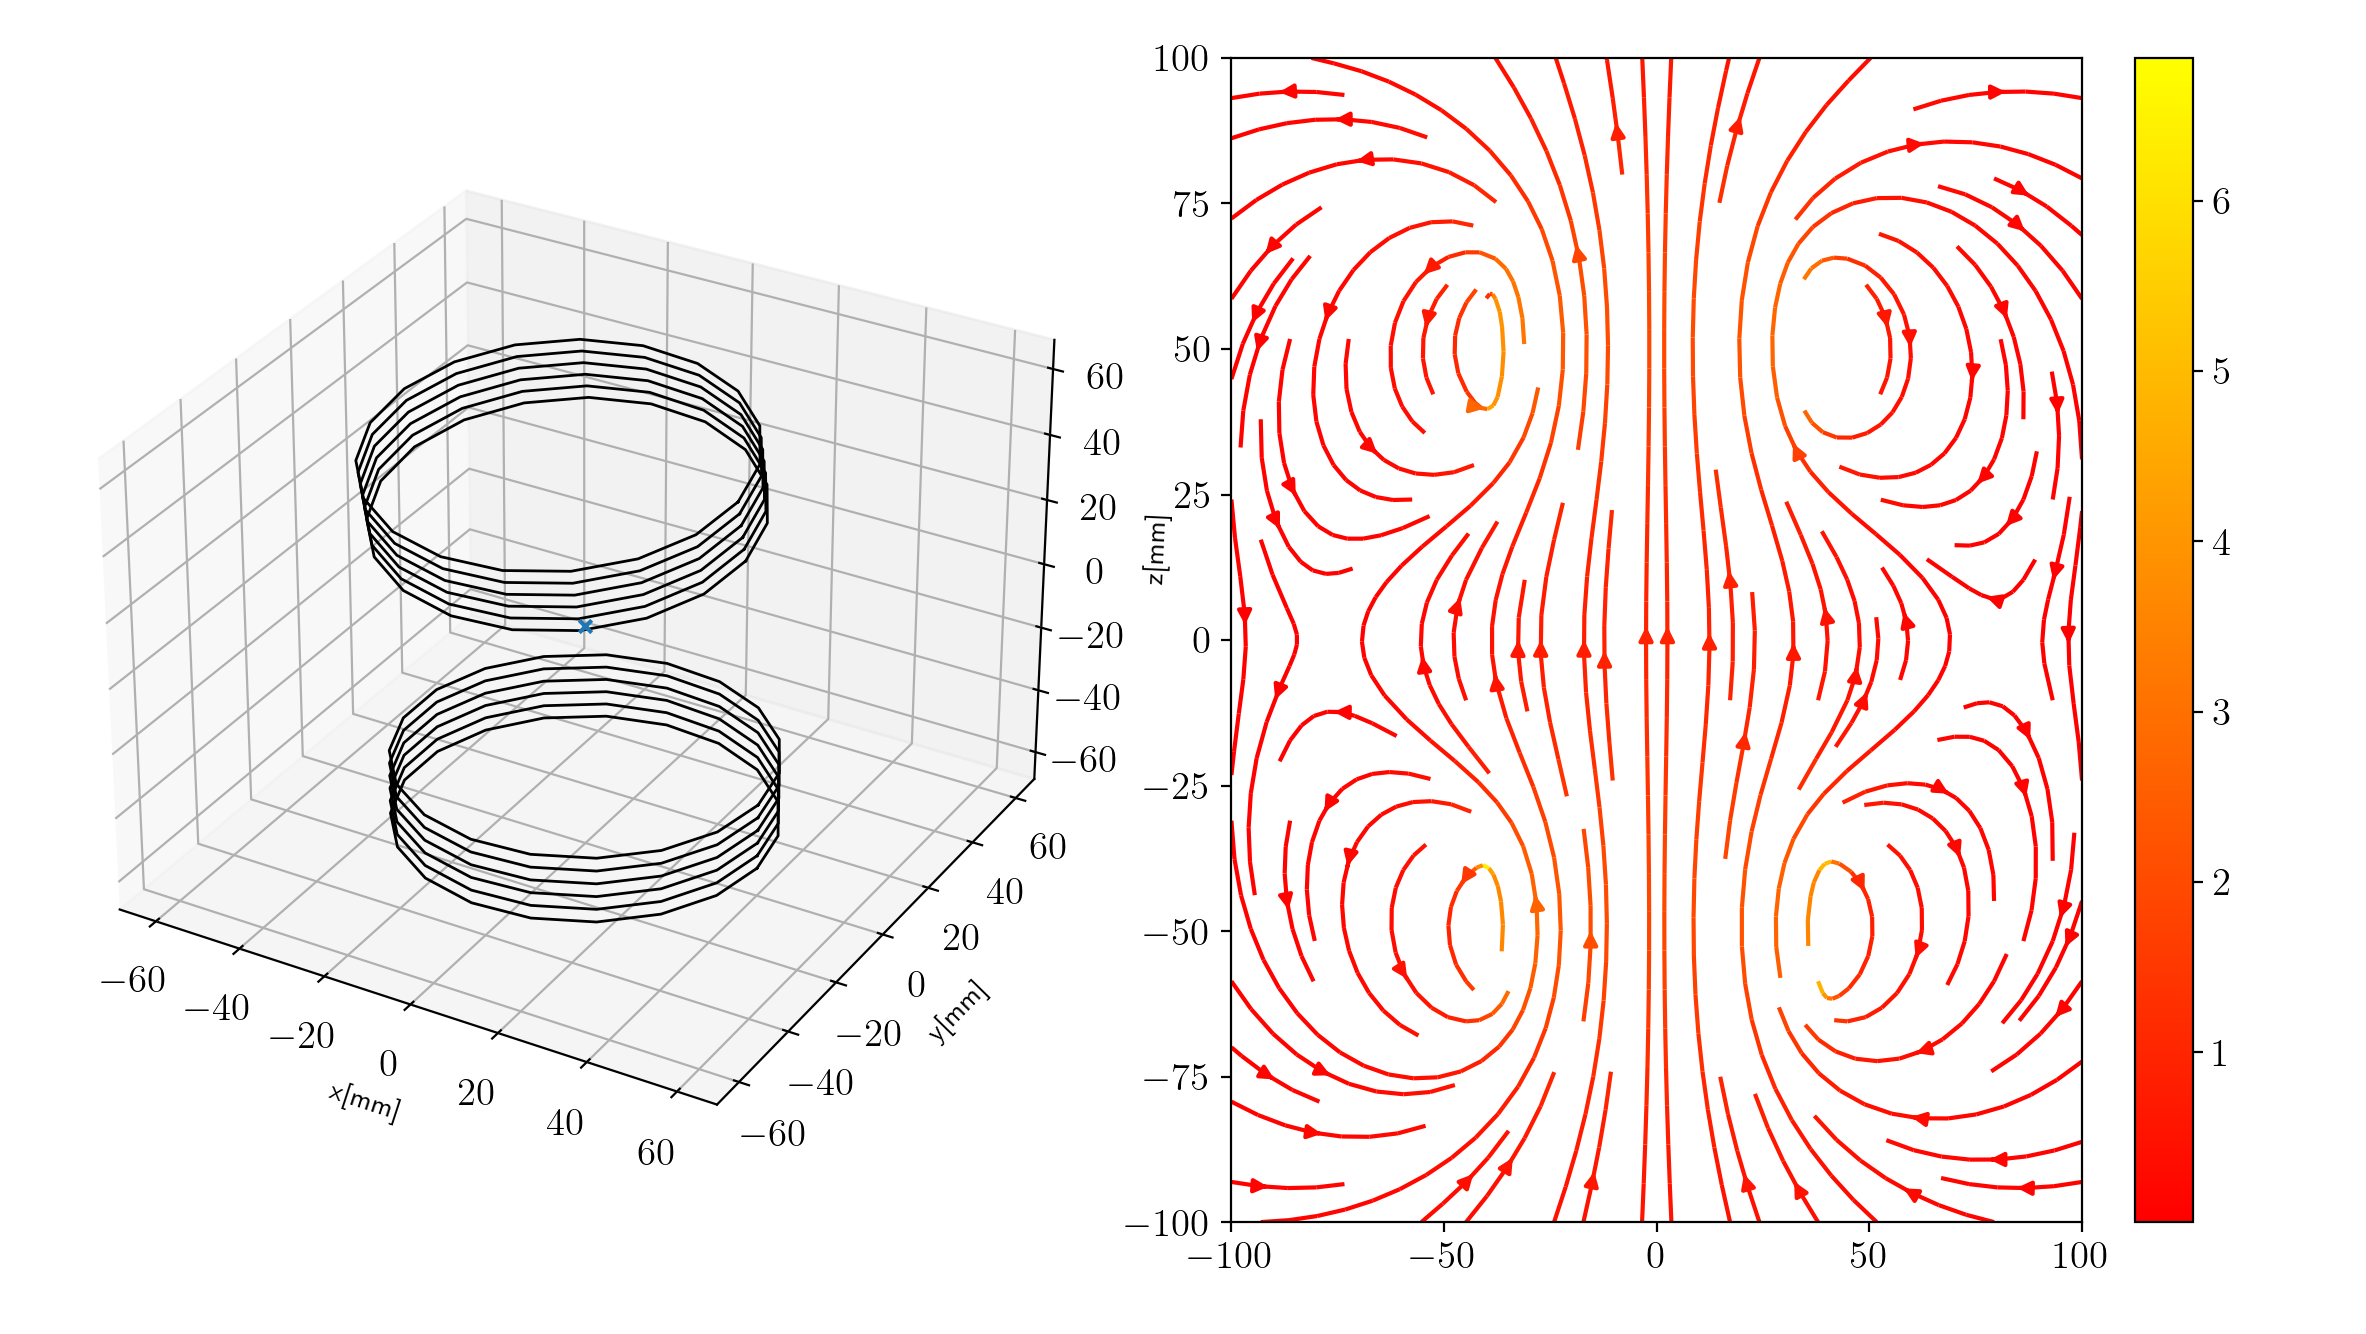
\includegraphics[width=\linewidth]{Tilted_coil_10Deg}
    \centering
    \caption{Tilted coil of 10 degrees.}
    \label{tilted_coil}
\end{figure}

\begin{figure}[t]
    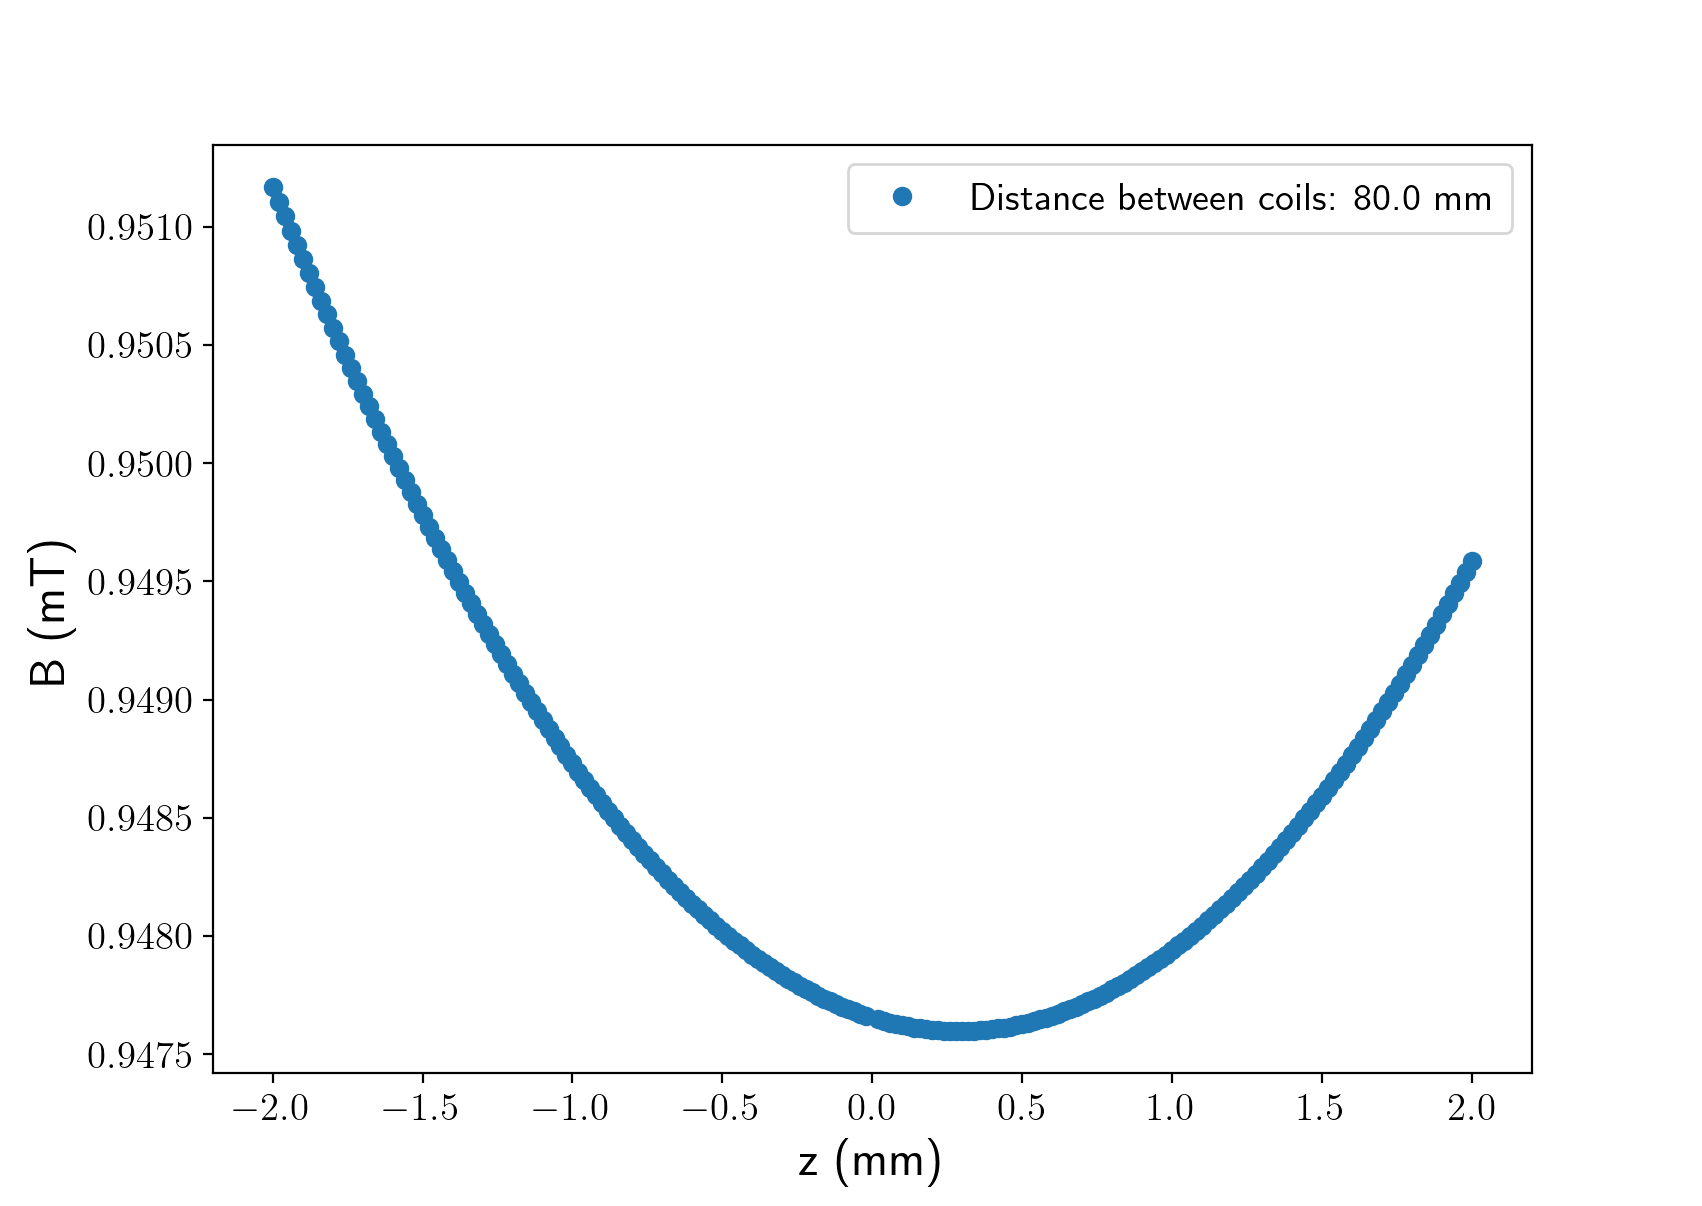
\includegraphics[width=\linewidth]{TiltedCoil10Deg_B}
    \centering
    \caption{Tilted coil of 10 degrees.}
    \label{tilted_coil_B}
\end{figure}

We can conclude that we don't need to worry too much about the exact geometry of the solenoid for homogenous magnetic field at the level of $\mu$T (or better than 0.1 Gauss), in this approximation and in the trapping region of about 0.15 mm. 

\clearpage
\newpage

\section{Heat dissipated on the coils}

Considering ideal coils with N turns copper wire with a given diameter, the resistance of the solenoid is given by:

\begin{equation}
    R_{solenoid} = \frac{L\rho}{\pi r_{wire}^{2}},
\end{equation}
where $\rho$ is the resistance of the copper, L is the length of the wire making the solenoid and $r_{wire}$ is the radius of the wire. The length of the wire can be approximated as $L = 2\pi \rho_{solenoid} N$, being $rho_{solenoid}$ the radius of each turn.

The total resistance of the solenoid is:

\begin{equation}
    R_{solenoid} = \frac{2 \rho_{solenoid} N \rho_{copper} I^{2}}{r_{wire}^{2}}
\end{equation}

The power dissipated is just $RI^{2}$ and as a scaling law:

\begin{equation}
    P \approx N (I / r_{wire})^{2}
\end{equation}

If we want to dissipate as minimum heat as we can, thicker wire and maximize the number of turns in the solenoid is desired. If the number of turn in the solenoid is increased by a factor of f then the dissipated power is reduced by a fact of f. Considering a 1.5 mm radius wire and $\rho_{copper} = 0.0171$ $\Omega$ mm $^{2}$/m, and a solenoid with 4 turns, that gives a total lentgh of about 1 m, a total resistance of about 2 m$\Omega$ and $I = 20$ A, then 1 W will be dissipated as heat on each solenoid.


\clearpage
\newpage
\section{Zeeman effect on $^{87}$Rb}
We turn now our attention to the calculation of the Zeeman shift on the energy levels of $^{87}$Rb. Two Hamiltonians will be of relevance: the hyperfine strutcture and the Zeeman effect. The hyperfine structure is simply given by:

\begin{equation}
    \mathcal{H}_{hfs} = A_{hfs} \vec{I} \cdot \vec{J} + B_{hfs} \frac{ 3 (\vec{I} \cdot \vec{J})^{2} + 3 \vec{I} \cdot \vec{J}/2 - I(I+1)J(J+1)}{2I(2I-1)J(2J-1)}
\end{equation}

The quantum numbers are the total angular momentum of the atom which, for a hydrogen-like system, would be just the several angular momentum of the outter electron. The above expression can be written in a simpler manner from the calculation point of view:

\begin{equation}
    \mathcal{H}_{hfs} = \frac{1}{2}A_{hfs} K + B_{hfs} \frac{ 3/2 K(K+1) - 2I(I+1)J(J+1)}{4I(2I-1)J(2J-1)}
\end{equation}
with $K = F(F+1) - I(I+1) - J(J+1)$. For the ground state 5S$_{1/2}$, only the first term is relvant and for this specific isotope, $I=3/2$. The usual quantum mechanics relation remains: $F = J + I$, $J = L + S$. For the ground state, there are two hyperfines levels, $F=1,2$ with the respective Zeeman sublevels that are degenerated for zero magnetic field. The hyperfine splitting can be calculated by extracting the eigenvalues of the Hamiltonian with the values:

\begin{center}
 \begin{tabular}{||c c c||} 
 \hline
 Magnetic dipole constant & A$_{5S_{1/2}}$ &  3.417 341 305 452 15(5) GHz  \\ 
 \hline
 Magnetic dipole constant & A$_{5P_{1/2}}$ &  408.328(15) MHz \\ 
 \hline
  Magnetic dipole constant & A$_{5P_{3/2}}$ &  84.7185(20) MHz \\ 
  \hline
  Electric Quadrupole constant & B$_{5P_{3/2}}$ &  12.4965(37) MHz \\ [1ex] 
 \hline
\end{tabular}
\end{center}

The ground state splitting is about 6.8 GHz. We now include in the Hamiltonian the contribution due to a non-zero magnetic field and for energy shift that are smaller than the fine structure splitting:

\begin{equation} \label{hz_high_field}
    \mathcal{H}_{z} = \mu_{B}B_{0} (g_{j} J_{z} + g_{I} I_{z})
\end{equation}

with, 

\begin{equation}
    g_{J} \sim 1 + \frac{J(J+1) + S(S+1) - L(L+1)}{2J(J+1)}
\end{equation}

For the condition where the Zeeman shift of the Zeeman sublevels is small compared to the hyperfine splitting between $F=2$ and $F=1$, we can consider these two level as being independent (or not mixed) and the calculation can be approximated to:

\begin{equation}
    \mathcal{H}_{z} = \mu_{B}B_{0} g_{f} m_{z}
\end{equation}

with,

\begin{equation}
    g_{F} \sim g{J} \frac{F(F+1) - I(I+1) + J(J+1)}{2F(F+1)}
\end{equation}

In this approximation, 

$$
\Delta\mathcal{E}_{z} = \left\{
    \begin{array}{ll}
        7 m_{f} \textrm{ MHz / mT}, F = 2 \\
        - 7 m_{f} \textrm{ MHz / mT}, F = 1
    \end{array}
\right.
$$

If we consider the qubit transition, for example, $\ket{5S_{1/2}, F=1, m_{f}=1}$ $\rightarrow$ $\ket{5S_{1/2}, F=2, m_{f}=2}$, this transition will be shifted by 21 MHz/mT. On the $\mu$T regime, this is about 21 kHz. 

Considering higher fields, then the Zeeman Hamiltonian will mix the states of F = 2 and F = 1 with the same m$_{f}$. In this case, we use the expression \ref{hz_high_field} and diagonalize $\mathcal{H}_{hfs} + \mathcal{H}_{z}$. On figure \ref{ZeemanShift_5S} the levels are displayed as a function of the magnetic field. We can see that, by considering the mix between the quantum states with different F's, the states with $m_{f} = 0$ starts to being shifted by the magnetic field at the level of 100 mT.

\begin{figure}[t]
    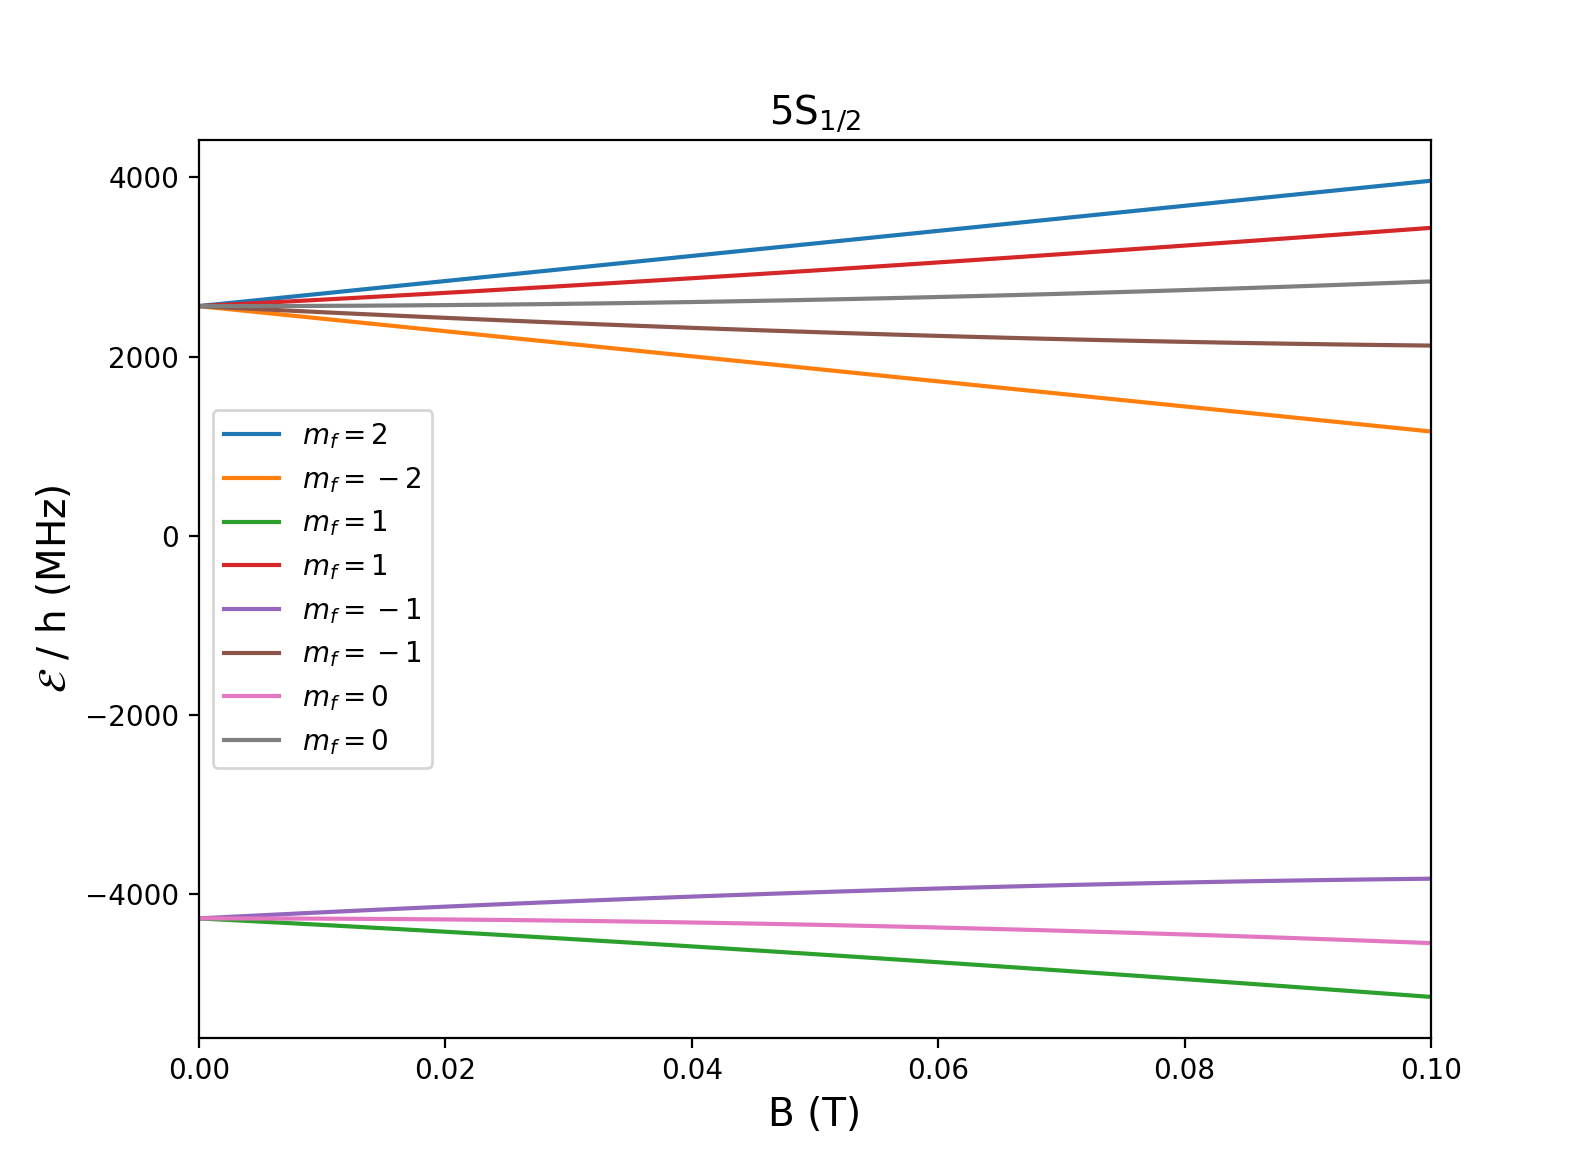
\includegraphics[width=\linewidth]{Zeeman_shift}
    \centering
    \caption{Energy levels of the 5S$_{1/2}$ level in a magnetic field.}
    \label{ZeemanShift_5S}
\end{figure}

\clearpage
\newpage



\section{Light shift on the atomic levels}

The trap lasers will perturb on the level of 1-10 MHz the atomic levels and hence the transitions. In this section I calculate the shift on the relevant states. Starting by the Hamiltonian of the system:

\begin{equation}
 	\mathcal{H}_{I} = e \vec{r} \cdot \vec{\epsilon}_{q} \mathcal{E}_{0}
 \end{equation} 
where q represents the polarization state of the trapping photons. From second order perturbation theory, the energy levels will be shifted by (energy shift already in Hz):

\begin{equation}
	\Delta \mathcal{E}_{i} = \sum_{j} \frac{\bra{j}\mathcal{H}_{I} \ket{i} }{ h (\nu_{i} - \nu_{j})}
\end{equation}

Now we can use the Wigner-Eckart theorem to break the calculation of the dipole matrix elements in several components:

\begin{equation}
	\bra{F', m_{f'}} er_{q} \ket{F, m_{f}} = \bra{F'} er_{q} \ket{F} \bra{F', m_{f'}} \ket{F, 1, m_{f} q}
\end{equation}

consisting of the reduced matrix and the Clebsch-Gordon coefficients, which can be written in terms of 3-j symbol:

...

\begin{equation}
	\Delta \mathcal{E}_{F m_{f}} = \frac{\mathcal{E}^{2}_{0}} {4h} \sum_{F', m_{f'}} \frac{\bra{F' m_{f'}} er_{q} \ket{F m_{f}} ^{2} }{ \nu_{laser} - (\nu_{F' m_{f'}} - \nu_{F m_{f}})}
\end{equation}

And the field amplitude can be calcuated in terms of laser power and waist:

\begin{equation}
	I = \frac{2P}{\pi \omega^{2}_{0}}
\end{equation}
and
\begin{equation}
	\mathcal{E}^{2}_{0} = \frac{2I}{\epsilon_{0} c}
\end{equation}
\clearpage
\newpage
\section{Quantum state preparation -- Optical pumping}

The goal is to initialize the qubits in a given state. Considering optical pumping techniques, it is chosen to prepare the atoms in the state $\ket{5S_{1/2}, F,m_{f} = 2,2}$ and the pumping scheme is shown on figure \ref{OpticalPumping}. The experiment starts with the atoms populating all the Zeeman levels in the ground hyperfine states. The optical pumping laser at 780 nm is prepared such that it addresses $\sigma^{+}$ transitions from $\ket{5S_{1/2}, F=2}$ $\rightarrow$ $\ket{5P_{3/2}, F=2}$ with $\Delta m_{f} = +1$. In this way, when the an atom populate the level $\ket{5S_{1/2}, F=2, m_{f}=2}$, the laser-atom interaction is stopped, avoiding unneccessary heating. 

The atoms initially populated in the $\ket{5S_{1/2}, F=1}$ are not excited by the optical pumping laser, being off resonance. In order to pump those atoms into the desired state, a repumper laser is used to pump those atoms in the $\ket{5P_{3/2}, F=2}$ and then they eventually decay to $\ket{5S_{1/2}, F=2}$ where they enter in the optical pumping system. 

\begin{figure}[t]
    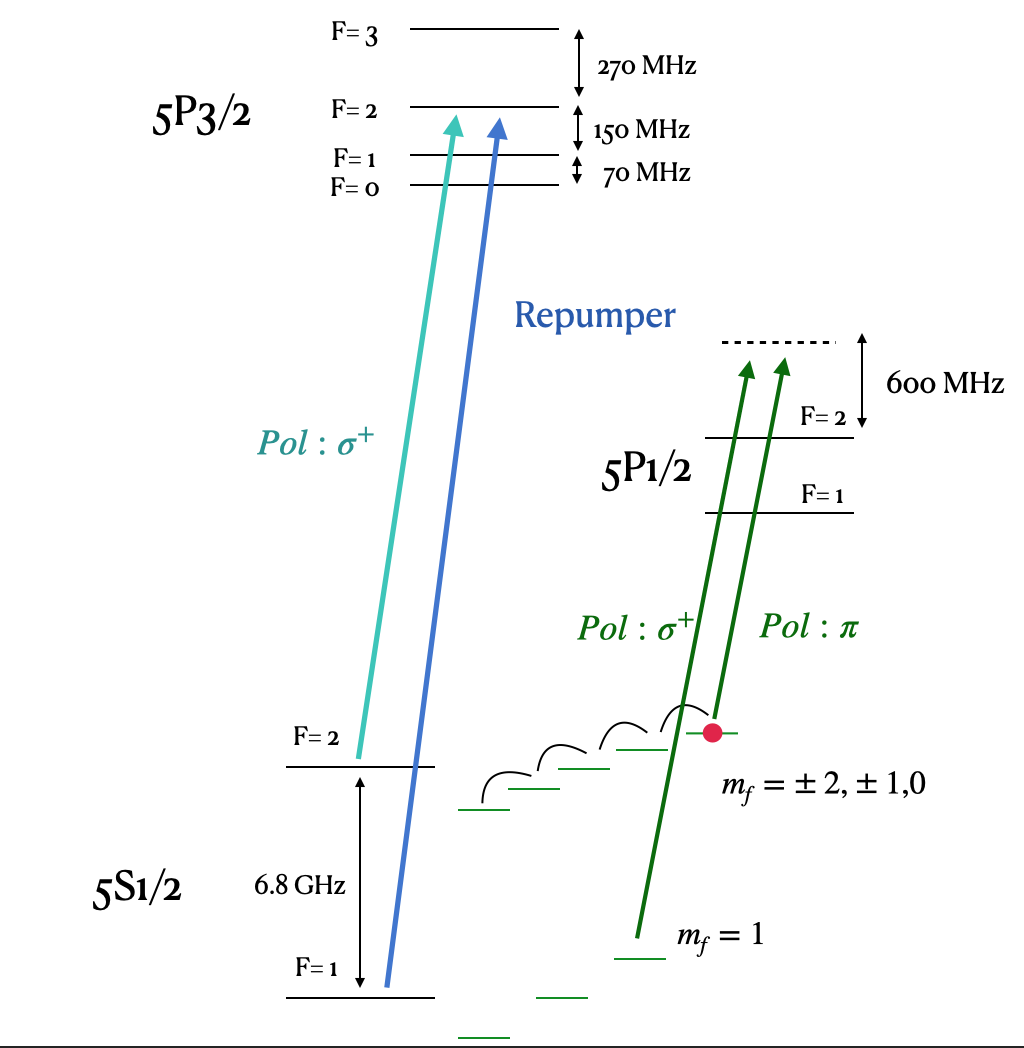
\includegraphics[width=0.8\linewidth]{OpticalPumpingScheme}
    \centering
    \caption{Optical pumping scheme to initialize the qubits in the $\ket{5S_{1/2}, F=2, m_{f}=2}$ state.}
    \label{OpticalPumping}
\end{figure}

The diagnostics is performed with a two-photons Raman transition connecting the qubit states with a 600 MHz detuning from the $5P_{1/2}$ transition at 795 nm. The scheme is shown on figure \ref{OpticalPumping}.




\end{document}